\documentclass[12pt]{article}
\usepackage{amsmath}
\usepackage{amssymb}
\usepackage{tikz}
\usepackage{pgfplots}
\usepackage{float}
\begin{document}
\title{Electrical Engineering 102, Homework 1}
\date{October 10th, 2018}
\author{Michael Wu\\UID: 404751542}
\maketitle

\section*{Problem 1}

The even component is shown below.
\begin{center}
	\begin{tikzpicture}[scale=0.8]
		\begin{axis}[ymin=-1.2,ymax=1.2,xmax=2.99,xmin=-2.99,axis lines = middle]
			\addplot[color=black,mark=none] coordinates {
				(-2,0)
				(-2,0.5)
				(-1,0)
				(-1,1)
				(1,1)
				(1,0)
				(2,0.5)
				(2,0)
			};
		\end{axis}
	\end{tikzpicture}
\end{center}
The odd component is shown below.
\begin{center}
	\begin{tikzpicture}[scale=0.8]
		\begin{axis}[ymin=-1.2,ymax=1.2,xmax=2.99,xmin=-2.99,axis lines = middle]
			\addplot[color=black,mark=none] coordinates {
				(-2,0)
				(-2,0.5)
				(-1,1)
				(-1,0)
				(1,0)
				(1,-1)
				(2,-0.5)
				(2,0)
			};
		\end{axis}
	\end{tikzpicture}
\end{center}
\section*{Problem 2}

\paragraph{a)}

\begin{enumerate}
	\item \(x(1-3t)\)
	\begin{center}
		\begin{tikzpicture}[scale=0.8]
			\begin{axis}[ymin=-1.2,ymax=1.2,xmax=2.99,xmin=-2.99,axis lines = middle]
				\addplot[color=black,mark=none] coordinates {
					(-.33333,0)
					(0,1)
					(0.33333,0)
					(0.33333,1)
					(2.99,1)
				};
			\end{axis}
		\end{tikzpicture}
	\end{center}
	\item \(x\left(\frac{t}{2}-2\right)\)
		\begin{center}
		\begin{tikzpicture}[scale=0.8]
			\begin{axis}[ymin=-1.2,ymax=1.2,xmax=8.99,xmin=-8.99,xtick distance = 2,axis lines = middle]
				\addplot[color=black,mark=none] coordinates {
					(-8.99,1)
					(4,1)
					(4,0)
					(6,1)
					(8,0)
				};
			\end{axis}
		\end{tikzpicture}
	\end{center}
\end{enumerate}

\paragraph{b)}

\[y(t)=z(-2t-2)\]

\section*{Problem 3}

\paragraph{a)}

\begin{enumerate}
	\item Periodic. The fundamental period is \(\pi\) and the fundamental frequency is \(\frac{1}{\pi}\).
	\item Periodic. The fundamental period is \(\sqrt{2}\) and the fundamental frequency is \(\frac{1}{\sqrt{2}}\).
	\item Periodic. The fundamental period is \(\frac{1}{3}\) and the fundamental frequency is \(3\).
	\item Not periodic. There is no common multiple between the periods of \(\pi\) and \(\sqrt{2}\).
	\item Periodic. The fundamental period is \(1\) and the fundamental frequency is \(1\).
	\item Not periodic. The exponential term makes it so that the amplitude of the sine wave is always decreasing with time.
	\item Not periodic. There is no common multiple between the periods of \(2\) and \(\sqrt{2}\).
\end{enumerate}

\paragraph{b)}

Assuming \(x(t)\) is continuous, \(x(0)=0\) because the function has rotational symmetry about the origin. Because it is periodic, it is also true that \(x(T_0)=x(0)\).
Thus \(x(T_0)=0\).

\paragraph{c)}

The even \(x_e(t)\) and odd \(x_o(t)\) components of a signal \(x(t)\) are unique and given by the following formulas.
\begin{gather*}
	x_e(t) = \frac{x(t)+x(-t)}{2}\\
	x_o(t) = \frac{x(t)-x(-t)}{2}
\end{gather*}
So if \(x(t)\) is periodic with a period of \(T\), we have that \(x(t+T)=x(t)\). Similarly we have \(x(t)=x(t-T)\). Then we can show the following.
\begin{gather*}
	x_e(t+T) = \frac{x(t+T)+x(-t-T)}{2} = \frac{x(t)+x(-t)}{2} = x_e(t)\\
	x_o(t+T) = \frac{x(t+T)-x(-t-T)}{2} = \frac{x(t)-x(-t)}{2} = x_o(t)
\end{gather*}
Therefore the even and odd components of \(x(t)\) must also be periodic.

\section*{Problem 4}

\paragraph{a)}

\begin{enumerate}
	\item Energy Signal. Since this signal is even, I can obtain its energy by evaluating the following integral.
	\[2\int_0^\infty e^{-2t}\,dt=\left.-e^{-2t}\right|_0^\infty=1\]
	Thus this signal has an energy of 1.
	\item This signal has infinite energy but zero power. Thus it is neither an energy signal nor a power signal. This is because integrating the
	signal squared has an antiderivative of \(\ln(x)\).
	\item Power Signal. It has a power of \(\frac{1}{2}\). This can be seen due to the exponential portion adding no power because it fades away. Then
	there is an average power of \(0\) before \(t=0\) and an average power of \(1\) afterwards for an average power of \(\frac{1}{2}\).
\end{enumerate}

\paragraph{b)}

\begin{align*}
	E_x&=\int_{-\infty}^\infty \left|x(t)\right|^2\,dt\\
	&=\int_{-\infty}^\infty \left(x_e(t)+x_o(t)\right)^2\,dt\\
	&=\int_{-\infty}^\infty x_e(t)^2+2x_e(t)x_o(t)+x_o(t)^2\,dt\\
	&=\int_{-\infty}^\infty x_e(t)^2\,dt + \int_{-\infty}^\infty 2x_e(t)x_o(t)\,dt + \int_{-\infty}^\infty x_o(t)^2\,dt\\
	&=E_{x_e}+0+E_{x_o}
\end{align*}

\pagebreak

\section*{Problem 5}

\paragraph{a)}

\begin{enumerate}
	\item
	\begin{align*}
		\frac{d}{d\theta} \sin(\theta) &= \frac{d}{d\theta} \frac{e^{j\theta}-e^{-j\theta}}{2j} \\
		&=\frac{e^{j\theta}+e^{-j\theta}}{2}\\
		&=\cos(\theta)
	\end{align*}
	\item
	\begin{align*}
		\sin^2(\theta) &=\left(\frac{e^{j\theta}-e^{-j\theta}}{2j}\right)^2 \\
		&=-\frac{e^{j2\theta}-2+e^{-j2\theta}}{4}\\
		&=\frac{1}{2}\left(1-\frac{e^{j2\theta}+e^{-j2\theta}}{2}\right)\\
		&=\frac{1}{2}(1-\cos(2\theta))
	\end{align*}
	\item
	\begin{align*}
		e^{j\alpha}+e^{j\beta} &=e^{j\frac{\alpha+\beta}{2}}\left(e^{j\frac{\alpha-\beta}{2}}+e^{j\frac{\beta-\alpha}{2}}\right) \\
		&=2e^{j\frac{\alpha+\beta}{2}}\left(\frac{e^{j\frac{\alpha-\beta}{2}}+e^{-j\frac{\alpha-\beta}{2}}}{2}\right)\\
		&=2e^{j\frac{\alpha+\beta}{2}}\cos\left(\frac{\alpha-\beta}{2}\right)
	\end{align*}
\end{enumerate}

\paragraph{b)}

\begin{enumerate}
	\item
	\begin{align*}
		-(1+j)e^{j(1+2t)}&=-(1+j)(\cos(1+2t)+j\sin(1+2t))\\
		&=-\cos(1+2t)+\sin(1+2t)\\
		&\qquad+j(-\cos(1+2t)-\sin(1+2t))
	\end{align*}
	The real part is \(-\cos(1+2t)+\sin(1+2t)\) and the imaginary part is \(-\cos(1+2t)-\sin(1+2t)\).
	\item The magnitude is \(|1+j|=\sqrt{(1+j)(1-j)}=\sqrt{2}\). We also have that
	\[-(1+j)e^{j(1+2t)}=\sqrt{2}e^{-j\frac{3\pi}{4}}e^{j(1+2t)}=\sqrt{2}e^{j\left(1-\frac{3\pi}{4}+2t\right)}\]
	So the phase is \(1-\frac{3\pi}{4}+2t\).
\end{enumerate}

\section*{Problem 6}

\paragraph{a)}

I plotted the function using the following code.
\begin{verbatim}
fplot(@(t) exp(-t.^2).*cos(2*pi.*t));
xlabel('t(sec)');
set(gcf,'color','w');
export_fig problem6a.pdf;
\end{verbatim}
\begin{figure}[H]
    \begin{center}
        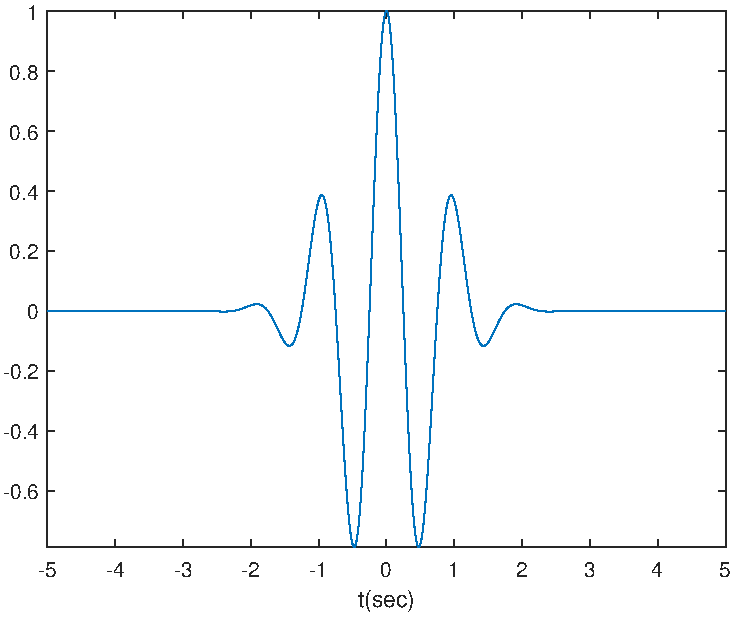
\includegraphics[width=2.56in]{problem6a.pdf}
    \end{center}
\end{figure}

\paragraph{b)}

I plotted the function using the following code.
\begin{verbatim}
x1=-2:0.01:1;
y1=ones(size(x1));
x2=1:0.01:2;
y2=x2-2;
plot(horzcat(x1,x2),horzcat(y1,y2));
xlabel('t(sec)');
ylim([-2 2]);
set(gcf,'color','w');
export_fig problem6b.pdf;
\end{verbatim}
\begin{figure}[H]
    \begin{center}
        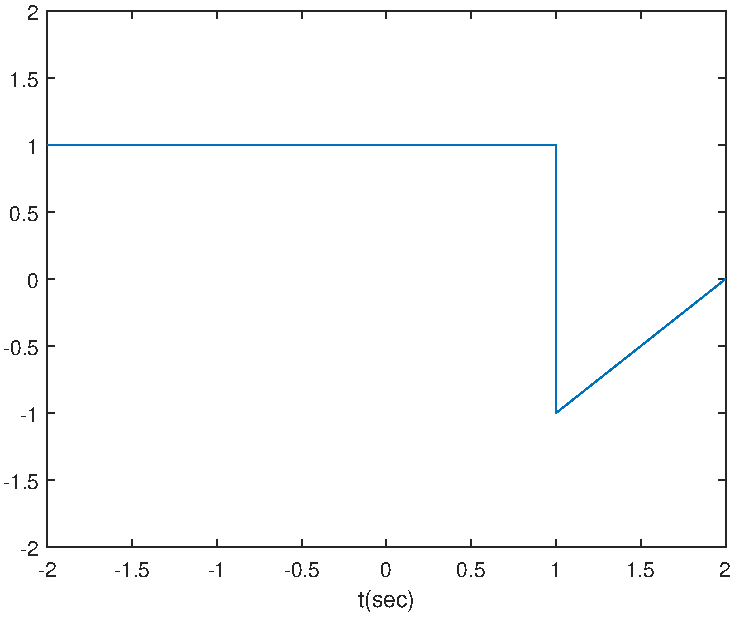
\includegraphics[width=2.5in]{problem6b.pdf}
    \end{center}
\end{figure}

\paragraph{c)}

I plotted the functions using the following code.
\begin{verbatim}
x1=-2:0.01:1;
y1=ones(size(x1));
x2=1:0.01:2;
y2=x2-2;
x=horzcat(x1,x2);
y=horzcat(y1,y2);
yrev=y(length(y):-1:1);
plot(x,(y+yrev)/2);
xlabel('t(sec)');
title('even component');
ylim([-2 2]);
set(gcf,'color','w');
export_fig problem6c-even.pdf;
plot(x,(y-yrev)/2);
xlabel('t(sec)');
title('odd component');
ylim([-2 2]);
export_fig problem6c-odd.pdf;
\end{verbatim}
\begin{figure}[H]
    \begin{center}
        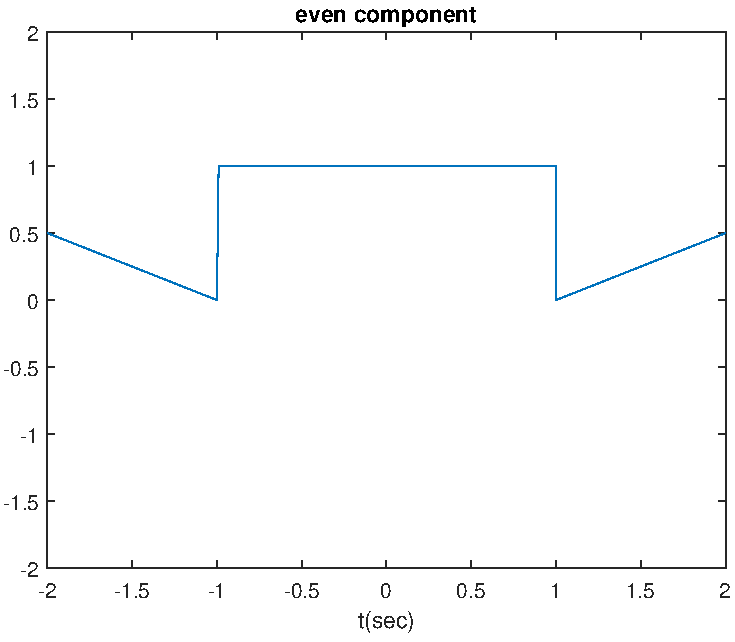
\includegraphics[width=2.5in]{problem6c-even.pdf}
		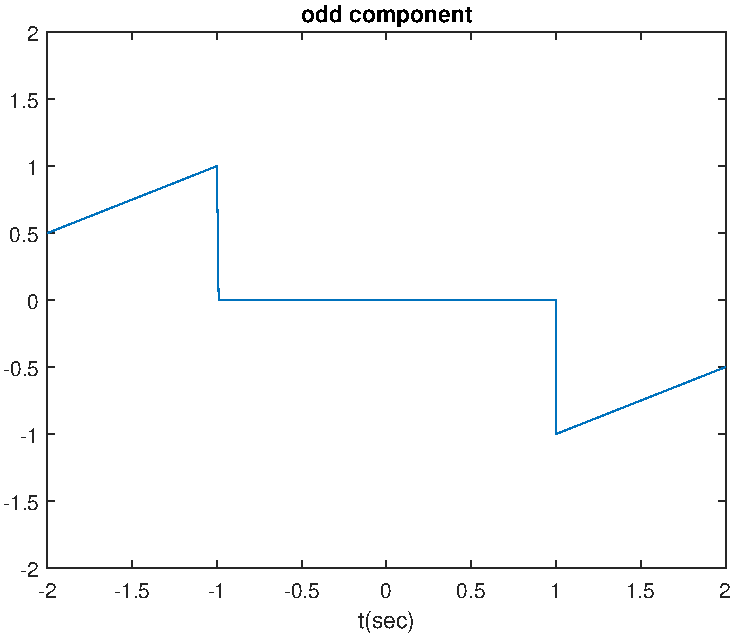
\includegraphics[width=2.5in]{problem6c-odd.pdf}
    \end{center}
\end{figure}

\paragraph{d)}

I plotted the functions using the following code.
\begin{verbatim}
t=-3:0.001:3;
y1=cos(2*pi.*t);
y2=cos(60*pi.*t);
y3=cos(2*pi.*t).*cos(60*pi.*t);
plot(t,y1);
xlabel('t(sec)');
title('cos(2\pit)');
set(gcf,'color','w');
export_fig problem6d-1.pdf;
plot(t,y2);
xlabel('t(sec)');
title('cos(60\pit)');
export_fig problem6d-2.pdf;
plot(t,y3);
xlabel('t(sec)');
title('cos(2\pit) cos(60\pit)');
export_fig problem6d-3.pdf;
\end{verbatim}
\begin{figure}[H]
    \begin{center}
        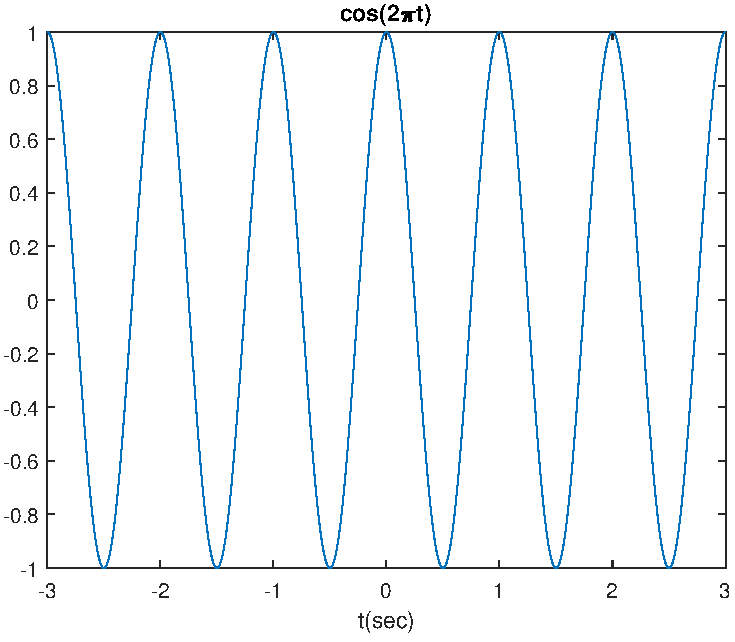
\includegraphics[width=2.5in]{problem6d-1.pdf}
		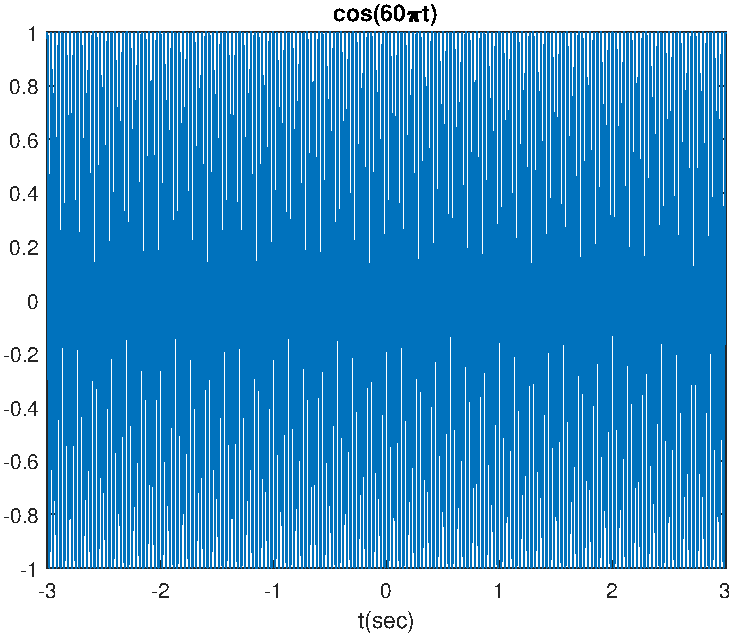
\includegraphics[width=2.5in]{problem6d-2.pdf}
		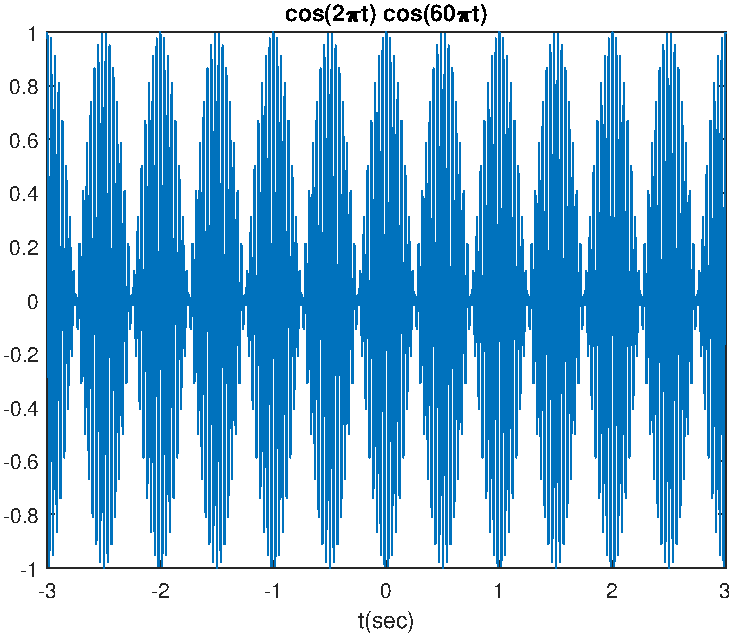
\includegraphics[width=2.5in]{problem6d-3.pdf}
    \end{center}
\end{figure}

\end{document}